\chapter{METODE PENELITIAN}
\label{sec:metode-penelitian}

\noindent Dalam penelitian ini akan dilakukan implementasi model Attention U-net untuk segmentasi mikrovaskular dalam WSI ginjal manusia sehat.  Penggunaan \textit{Aattention Gate} (AG) pada U-net dipilih untuk memusatkan perhatian model pada \textit{feature} yang berpengaruh dari \textit{encoder} ,sehingga bisa meningkatkan peforma model dalam tugas segmentasi mikrovaskular dalam WSI ginjal manusia sehat. Penelitian ini melibatkan beberapa tahapan mulai dari penginputan data sampai ke evaluasi model. Secara mendetail seluruh proses dari penelitian ini bisa dilihat pada flowchart berikut ini:
\begin{figure}[H]
	\centering
	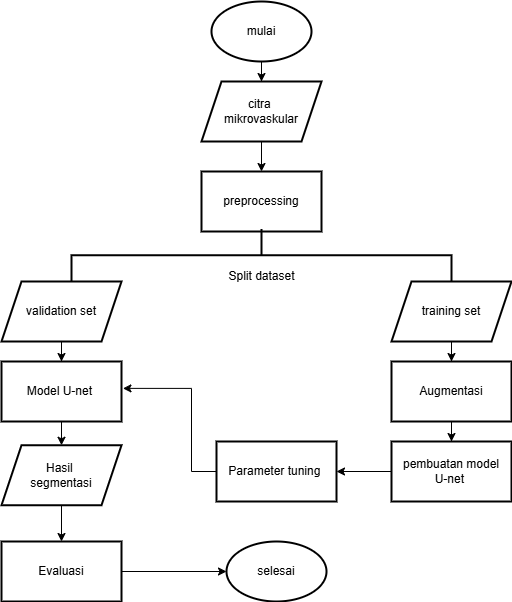
\includegraphics[scale=.6]{gambar/flow-chart.png}
	\caption{Flow chart Penerapan U-net}
	\label{fig:flow-chart}
\end{figure}

\section{Dataset Penelitian}

\noindent Dataset yang digunakan pada penelitian ini adalah data yang telah disediakan \textit{Human BioMolecular Atlas Program }(HuBMAP) di Kaggle: \url{https://www.kaggle.com/competitions/hubmap-organ-segmentation}\cite{howard_hubmap_2023}.  Data ini berisi citra WSL mikrovaskular ginjal manusia yang telah diwarnai menggunakan metode \textit{2D PAS-stained}. \textit{2D PAS-stained} mengacu pada citra dua dimensi yang diwarnai menggunakan pewarnaan Periodic Acid-Schiff (PAS). Data ini terdiri dari 7033 citra yang telah diwarnai dengan format TIFF beresolusi 512x512 dimana 1633 telah dianotasikan ke tiga kelas yakni, \textit{blood vessels}(pembuluh darah), \textit{glomelurus} dan \textit{unsure}(dikeragui).  Anotasi dari data tersebut disimpan dalam file json yang merepresentasikan kordinat mask poligon yang sesuai dengan area setiap kelas pada gambar. Dalam penelitian ini hanya data yang telah dianotasikan saja yang akan digunakan untuk melatih model dengan menggabungkan ketiga kelas anotasi menjadi satu kelas mikrovaskular.

\begin{figure}[H]
	\centering
	\begin{subfigure}[b]{0.3\textwidth}
		\centering
		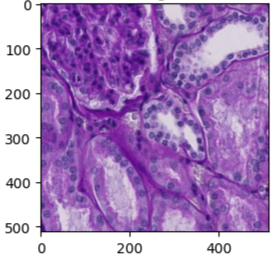
\includegraphics[width=\textwidth]{gambar/image.png}
		\caption{Image}
		\label{fig:image}
	\end{subfigure}
	\hfill
	\begin{subfigure}[b]{0.3\textwidth}
		\centering
		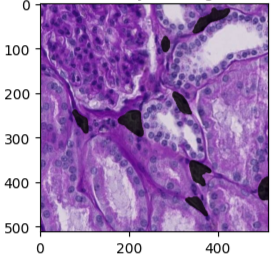
\includegraphics[width=\textwidth]{gambar/overlayed_image.png}
		\caption{Ovelayed image}
		\label{fig:overlayed-image}
	\end{subfigure}
	\hfill
	\begin{subfigure}[b]{0.3\textwidth}
		\centering
		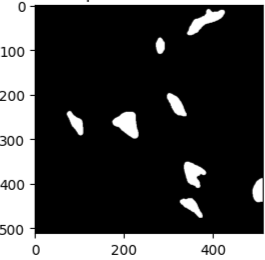
\includegraphics[width=\textwidth]{gambar/pixelwise_label.png}
		\caption{Pixel wise label}
		\label{fig:Pixel wise label}
	\end{subfigure}
	\caption{Sample WSI yang telah dianotasikan}
	\label{fig:sample_data}
\end{figure}

\section{Spesifikasi Perangkat}

\noindent Penelitian ini akan dilakukan di lingkungan komputasi remote menggunakan \textit{Kaggle Notebooks}. Kaggle menyediakan perangkat keras yang diperlukan dalam penelitian, sehingga peneliti bisa fokus pada eksekusi teori ke dalam kode python tanpa perlu konfigurasi perangkat terlebih dahulu. Spesifikasi sumber daya komputasi yang disediakan Kaggle bisa dilihat pada tabel \ref{tab:cpu_specs}.
\begin{table}[h]
	\centering
	\caption{Spesifikasi CPU pada Lingkungan Komputasi Remote Kaggle Notebook.}
	\label{tab:cpu_specs}
	\begin{tabular}{lllll}
		\hline
		\textbf{Jenis} & \textbf{CPU}  & \textbf{Core CPU} & \textbf{RAM} & \textbf{GPU}      \\ \hline
		CPU            & Default       & 4                 & 30 GB        & -                 \\
		GPU P100       & Intel Skylake & 4                 & 29 GB        & 2 Nvidia Tesla T4 \\
		TPU 1VM        & -             & 96                & 330 GB       & -                 \\ \hline
	\end{tabular}
\end{table}

\noindent \textit{Notebook} yang menggunakan \textit{Central Processing Unit }(CPU) dan \textit{Graphics Processing Unit} (GPU) memiliki waktu eksekusi selama 12 jam, sedangkan notebook yang menggunakan \textit{Tensor Processing Unit} (TPU) memiliki waktu eksekusi selama 9 jam. Tersedia 20 \textit{Gigabytes} ruang penyimpanan otomatis direktori '/kaggle/working' dan ruang penyimpanan \textit{scratchpad} tambahan yang tidak akan disimpan diluar sesi saat ini.


\section{Preproccessing}

\noindent \textit{Preproccessing} merupakan langkah penting dalam mempersiapkan dataset agar bisa gunakan dalam pelatihan dan evaluasi model. Langkah-langkah yang biasanya dilakukan dalam \textit{preproccessing} citra biomedis untuk tugas segmentasi adalah: normalisasi, augmentasi, dan pembagian dataset menjadi data latih dan validasi.

\subsection{Normalisasi}

\noindent Dalam tahap ini, intensitas piksel dari gambar yang biasanya dalam rentang 0 hingga 225 akan di ubah menjadi rentang lebih kecil seperti 0 dan 1. Proses ini bisa mempercepat proses konvergensi model dan meningkatkan akurasi model. Berikut adalah formula untuk normalisasi intensitas piksel dalam gambar:

\begin{equation}
	x' = \frac{x - \min}{\max - \min}
\end{equation}

\noindent
keterangan:
\begin{itemize}
	\item $x$ : nilai piksel asli
	\item $\min$ : nilai minimum dari piksel
	\item $\max$ : nilai maksimum dari piksel
\end{itemize}


\subsection{Pembagian dataset}

\noindent Dalam pengembangan model deep learning pembagian dataset merupakan sebuah langkah yang penting. Dalam langkah ini dataset akan dibagi menjadi set latih dan set uji. Perlakuan ini akan meningkatkan keakuratan evaluasi pada model dengan memastikan model tidak hanya diuji pada data yang telah dilihat selama pelatihan. Rasio pembagian yang digunakan dalam penelitian ini adalah \(80:20\), dimana 80\% data digunakan sebagai set latih dan 20\% data digunakan sebagai set uji. Pembagian ini akan mengambil data secara acak dari seluruh data yang telah dianotasikan saja. 

\subsection{Augmentasi}

\noindent Proses ini merupakan teknik untuk megenerasi  data yang mirip dengan data original namun berbeda pada pandangan model. Pada penelitian ini akan dilakukan augmentasi berupa transformasi geometri secara acak seperti: rotation (rotasi), scaling(skala) dan flipping(membalikkan).

\subsection{Konversi Grayscale}
\noindent Konversi grayscale adalah proses mengubah gambar berwarna (RGB) menjadi gambar hitam-putih (grayscale). Ini melibatkan penghilangan informasi warna dan hanya mempertahankan intensitas cahaya, yang mengubah setiap piksel gambar menjadi nilai intensitas tunggal, sehinggaa model bisa fokus pada struktur tanpa gangguan fitur warna. Konversi graysclale pada gambar menggunakan rumus berikut:
    \begin{equation}
	\text{Gray} = 0.2989 \times \text{Red} + 0.5870 \times \text{Green} + 0.1140 \times \text{Blue}
\end{equation}




\section{Pelatihan}
\noindent Pada tahap pelatihan ini, citra input beserta anotasinya akan digunakan untuk melatih model Attention U-net yang dikembangkan beserta U-net yang akan digunakan sebagai perbandingan peforma. Setiap arsitektur diuji dengan dua jenis optimizer, yaitu Adam dan \textit{Stochastic Gradient Descent (SGD)}, untuk mengevaluasi kinerja segmentasi mikrovaskular ginjal manusia pada setiap kombinasi model dan optimizer.

Proses pelatihan dilakukan dengan menggunakan kombinasi fungsi loss \textit{cross entropy} dan \textit{Dice coefficient loss} untuk menangani ketidakseimbangan kelas pada data. Selain itu, teknik oversampling diterapkan pada kelas minoritas untuk meningkatkan proporsi sampel minoritas di dalam batch data.

Untuk setiap kombinasi model dan optimizer, dilakukan variasi batch size sebesar 4, 8, dan 16 untuk menentukan ukuran batch yang memberikan hasil \textit{Dice Similarity Coefficient (DSC)} terbaik. Ukuran batch yang menghasilkan DSC tertinggi pada tahap awal ini kemudian dipilih sebagai batch size utama dan digunakan kembali dalam teknik oversampling guna memastikan konsistensi performa.

Penyesuaian laju pembelajaran (\textit{learning rate}) dilakukan secara otomatis menggunakan \textit{Reduce on Plateau callback}, sehingga tidak perlu divariasikan secara manual. Selain itu, pelatihan dihentikan secara dini menggunakan \textit{early stopping callback} yang memantau performa model pada data validasi, sehingga jumlah epoch tidak perlu ditentukan secara spesifik.

Berikut adalah tabel konfigurasi hyperparameter yang digunakan dalam pelatihan:

\begin{table}[h]
	\centering
	\caption{Variasi hyperparameter dalam pelatihan model.}
	\label{tab:hyperparameter}
	\begin{tabular}{lllll}
		\hline
		\textbf{Hyperparameter} & \multicolumn{4}{l}{\textbf{Variasi}}                  \\ \hline
		Arsitektur Model        & \multicolumn{4}{l}{Attention U-net, U-net}            \\
		Optimizer               & \multicolumn{4}{l}{Adam, SGD}                         \\
		Batch size              & \multicolumn{4}{l}{4, 8, 16}                          \\
		Epotch                  & \multicolumn{4}{l}{Ditentukan oleh \textit{early stopping}}    \\
		Learning rate           & \multicolumn{4}{l}{Ditentukan oleh \textit{Reduce on Plateau}} \\ \hline
	\end{tabular}
\end{table}


\section{Evaluasi}

\noindent Tahap evaluasi dilakukan untuk menilai kinerja model segmentasi dalam mendeteksi struktur mikrovaskular ginjal. Evaluasi ini dilakukan dengan menggunakan beberapa metrik yang sering digunakan dalam tugas segmentasi, yaitu \textit{precision}, \textit{recall}, \textit{intersection over union} (IoU), dan \textit{dice similarity coefficient} (DSC) \cite{jiang_iu-net_2023}. Metrik-metrik ini dipilih karena mampu memberikan gambaran kuantitatif mengenai akurasi dan kualitas hasil segmentasi yang dihasilkan oleh model terhadap \textit{ground truth}.

\begin{itemize}
	\item \textbf{Precision}: Precision mengukur proporsi area yang terdeteksi sebagai mikrovaskular yang benar-benar termasuk dalam kategori tersebut. Precision yang tinggi menunjukkan bahwa model mampu mengurangi \textit{false positives} dalam prediksi segmentasi.
	
	\item \textbf{Recall}: Recall mengukur kemampuan model dalam mendeteksi area mikrovaskular secara menyeluruh. Nilai recall yang tinggi menunjukkan bahwa model berhasil menemukan sebagian besar area yang benar-benar termasuk dalam struktur mikrovaskular, dengan meminimalkan \textit{false negatives}.
	
	\item \textbf{Intersection over Union (IoU)}: IoU mengukur tingkat tumpang tindih antara hasil segmentasi dan \textit{ground truth}. Nilai IoU yang mendekati 1 menunjukkan tingkat akurasi spasial yang tinggi, dengan segmentasi yang dihasilkan model sangat mirip dengan \textit{ground truth}.
	
	\item \textbf{Dice Similarity Coefficient (DSC)}: DSC merupakan metrik yang sering digunakan untuk menilai kualitas segmentasi, karena memberikan bobot yang sama pada precision dan recall. DSC juga mengukur kemiripan antara hasil segmentasi dan \textit{ground truth}, di mana nilai yang mendekati 1 menunjukkan bahwa hasil segmentasi sangat mendekati area yang diharapkan.
\end{itemize}

Secara keseluruhan, semakin tinggi nilai precision, recall, IoU, dan DSC, maka semakin baik kinerja model dalam melakukan segmentasi struktur mikrovaskular ginjal. IoU dan DSC, khususnya, digunakan sebagai metrik utama untuk mengevaluasi tingkat kemiripan antara hasil segmentasi dan \textit{ground truth}, di mana semakin mendekati nilai 1, maka semakin baik prediksi yang dihasilkan oleh model.







% Baris ini digunakan untuk membantu dalam melakukan sitasi
% Karena diapit dengan comment, maka baris ini akan diabaikan
% oleh compiler LaTeX.
\begin{comment}
\bibliography{daftar-pustaka}
\end{comment}
